\section{チェレンコフ放射}
チェレンコフ放射とは、荷電粒子が物質を通過する際に荷電粒子の速度がその物質中の光速を超えると光を発生する現象である。
またその光をチェレンコフ光という。
速度$\beta$の荷電粒子が屈折率$n$の物質中を通過する際に、チェレンコフ放射が発生する条件は$(\ref{eq:cherenkov_condition})$式で表せる。
\begin{equation}
  \label{eq:cherenkov_condition}
  \beta > \frac{1}{n}
\end{equation}
チェレンコフ光は図$\ref{fig:cherenkov}$のように円錐状に発生し、その際のチェレンコフ角$\theta_{c}$は$(\ref{eq:cherenkov_angle})$式のように表せる。
\begin{equation}
  \label{eq:cherenkov_angle}
  \cos \theta_{c} = \frac{1}{n\beta}
\end{equation}
また、単位長さの輻射体から発生するチェレンコフ光の光子数$dN/dx$は$(\ref{eq:cherenkov_light_yield})$式のように表される。
\begin{equation}
  \label{eq:cherenkov_light_yield}
  \frac{dN}{dx} = 2 \pi z^2 \alpha \int{\left(1-\frac{1}{\beta^2 n^2}\right)\frac{d\lambda}{\lambda^2}}
\end{equation}
ここで、$z$は荷電粒子の電荷数、$\alpha$は微細構造定数、$\lambda$はチェレンコフ光の波長である。
\begin{figure}[htbp]
  \centering
  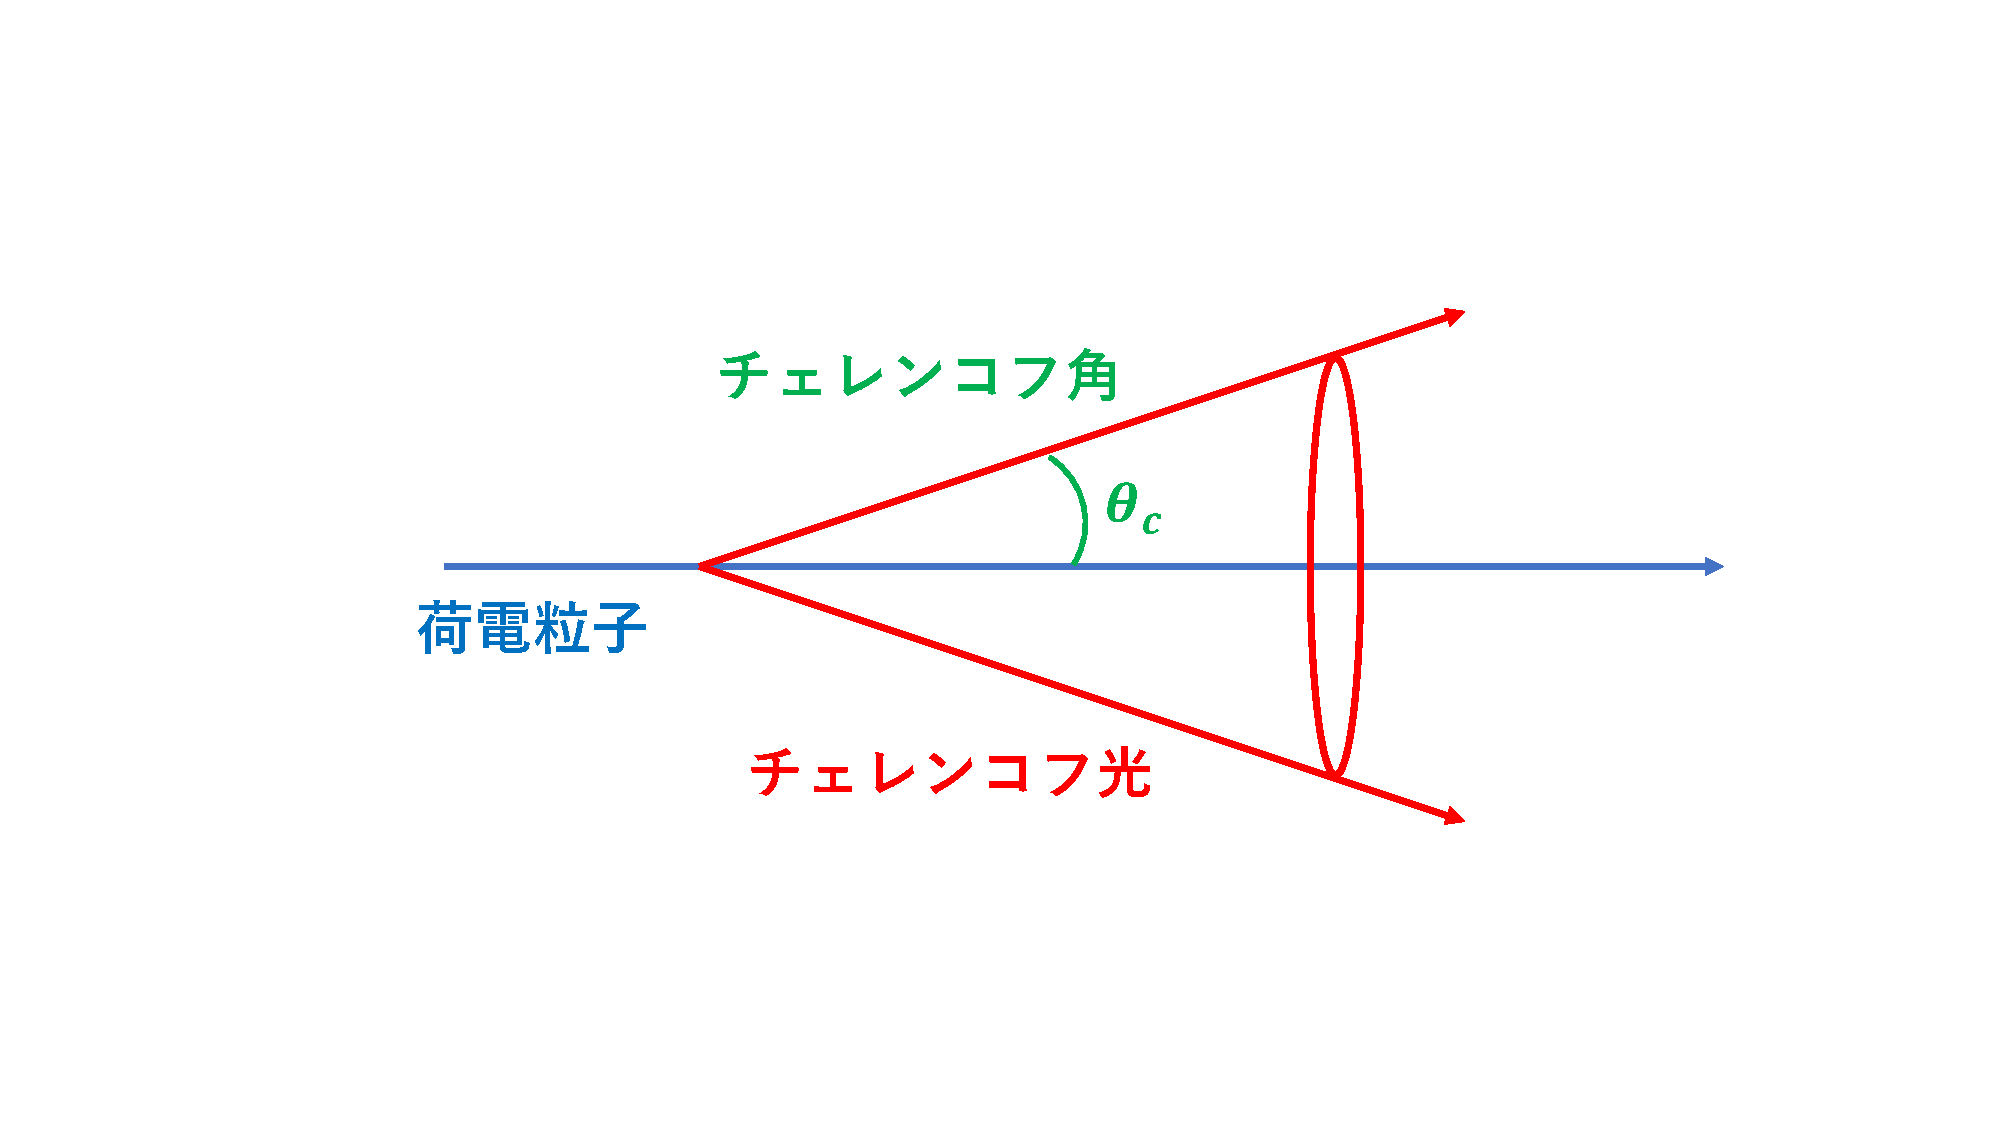
\includegraphics[width=10cm]{images/chapter2/cherenkov.pdf}
  \caption[チェレンコフ放射の模式図]{チェレンコフ放射の模式図。}\label{fig:cherenkov}
\end{figure}
